\chapter{Normalisation fit}
\label{sec:Normalisationfit}
This chapter describes the analysis of the normalisation channel \LbToLcmunu (\LcTopKpi) resulting in the signal yield \NLc for the calculation of \R. The method is different to the one in the signal channel \LbToDpmunuX due to several reasons:
The final state particles of the subdecay \LcTopKpi are all reconstructed. 
It is thus possible to see a clear \Lc mass peak as shown in figure \ref{fig:plot_Lc_M}.
The small sidebands indicate a small combinatorial background concerning the subdecay \LcTopKpi.
Background coming from a random combination of a \Lc with a muon can be estimated by a look at the WS final states combinations \Lc\mup.
Since a \Lb can't decay into a \Lc\mup due to charge conservation, this unphysical combination gives a good hint for randomly combined \Lc\mun.
The second reason why a different method is chosen compared to the \LbToDpmunuX channel is the fact that the \Lb can decay in several excited \Lc states (in the following denoted as \Lcstar for any excited \Lc state).
It has been shown in \ref{SL_Vub} that the \LbToLcmunu data is saturated by the decays \decay{\Lb}{\LcstarRes{(2595)}\mun\neumb} and \decay{\Lb}{\LcstarRes{(2625)}\mun\neumb}.
These excited \Lcstar instantly decay for instance in \Lc\pip\pim. 
If these two pions aren't reconstructed, this decay can't be distinguished by its topology.
That's why a different approach for the determination of \NLc has to be chosen.
The solution of the latter problem is to fit the corrected \pKpi\mun, i.e the visible \Lb mass.
An explanation for this choice and the description of the fit is given in section \ref{sec:Normalisationfit}.
\begin{figure}[hptb]
    \centering
	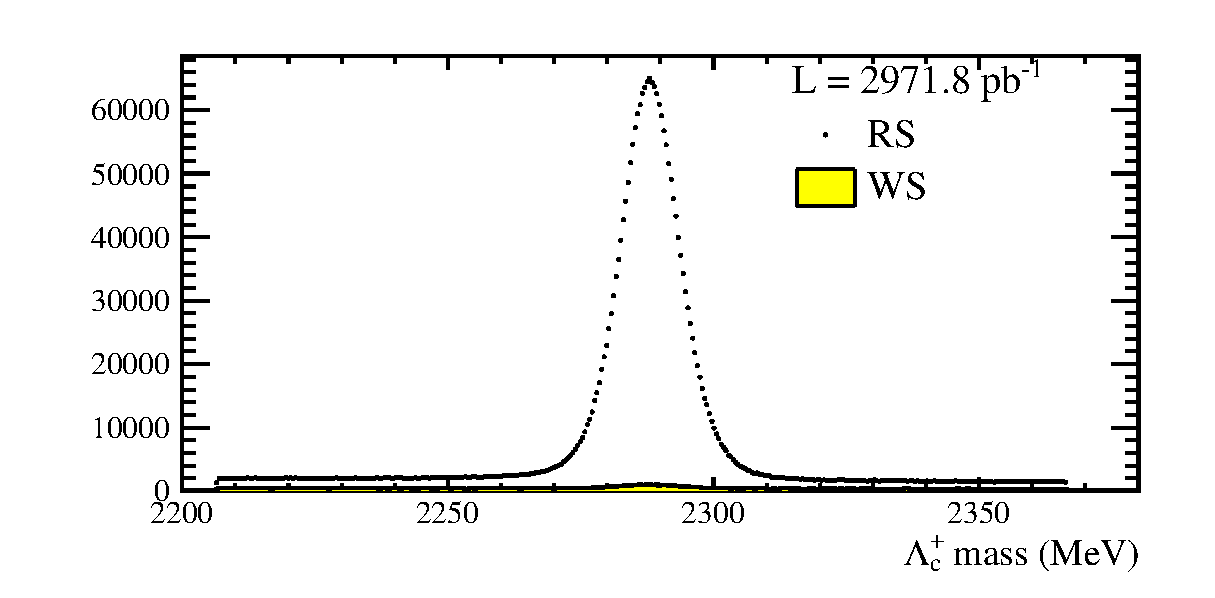
\includegraphics[width=\textwidth]{LbToLc/plots/data/Lc_M}	
	\caption{Plot of the invariant \pKpi mass. A clear mass peak identified as the \Lc can be seen. The yellow shaded area shows events with the WS combination \Lc\mup.}
	\label{fig:plot_Lc_M}
\end{figure}


\section{Reduction and handling of backgrounds}
This section describes the ways, how different sources of backgrounds are either handled or reduced.

\subsection{Non \Lc background}
As already mentioned the reconstructed \pKpi mass delivers a nice peak forming the hadronically decaying \Lc nicely seen in figure \ref{fig:plot_Lc_M}. 
Events being outside of this peak can be explained by a random combination of proton, kaon and pion and thus not being decay remnants of the \Lc.
Nonetheless there is also a certain amount of this ``combinatoric" background in the peak region.
It is statistically eliminated by a sideband subtraction (see section \ref{sec:Sidebandsubtraction}).
As signal band the invariant \pKpi masses in the range M(\pKpi) $\in \left[2260, 2320\right]\mev$ are chosen.
The background bands are M(\pKpi) $\in \left[2225, 2260\right]\mev$ or M(\pKpi) $\in \left[2320, 2345\right]\mev$.

\subsection{Random combinations of \Lc and \mun}
The next possible source of backgrounds are random combinations of \Lc and \mun. 
Due to the semileptonic decay \LbToLcmunu and hence the missing neutrino \neumb it is not possible to use a sidebandsubtraction on the invariant \pKpi\mun (\Lc\mun) mass.
Thus, wrong sign (WS) events, i.e. ``unphysical" events with a \Lc\mup in the final state as explained above are used to estimate the amount of random \Lc\mun background.
While trying to perform the final fit later (see sec. \ref{sec:FitCorrectedMass}) it turns out, that the number of WS events is too small that the fit is sensitive to it.
As a consequence it is assumed that the shape and the number of the WS events are equal to the shape and number of random \Lc\mun combinations.
Finally, the WS events are subtracted from the ``right sign" (RS) events to eliminate this source of backgrounds.

\subsection{Peaking backgrounds}
The third source of backgrounds is peaking background from partially reconstructed decays. 
In this case the data is saturated by the decays \decay{\Lb}{\LcstarRes{(2595)}\mun\neumb} and \decay{\Lb}{\LcstarRes{(2625)}\mun\neumb} \cite{SL_Vub}.
The \Lcstar subsequently decay in a \Lc and an untracked neutral remnant, e.g. \piz, \pip\pim.
Since this decay happens instantly it looks the same as \LcTopKpi in the detector.
The solution is to fit the corrected \pKpi\mun (alias the visible \Lb) mass. 
A property of the corrected mass is that if the only missing particle is a massless, then the corrected mass should peak around the real mass of the mother particle, here the \Lb.
If there are additionally more missing, but massive particles then this peak should be shifted to lower masses.
It is thus expected that the corrected \pKpi\mun mass distributions look different for the semileptonic \Lb decays into a \Lc, \LcstarRes{(2595)} and \LcstarRes{(2625)}.
A fit of the corrected mass should also be able to distinguish between those components.

\section{Fit of the \pKpi\mun corrected mass}
\label{sec:FitCorrectedMass}
Having read the previous sections it should be clear, why the corrected \pKpi\mun mass is used for the determination of \NLc, the \LbToLcmunu signal yield.
Nonetheless it should be verified, that the corrected \pKpi\mun mass is an appropriate variable.
Therefore simulations for the different components, \LbToLcmunu, \decay{\Lb}{\LcstarRes{(2595)}\mun\neumb} and \decay{\Lb}{\LcstarRes{(2625)}\mun\neumb} are used to compare their corrected \pKpi\mun mass shapes.
\begin{figure}[hptb]
	\centering
	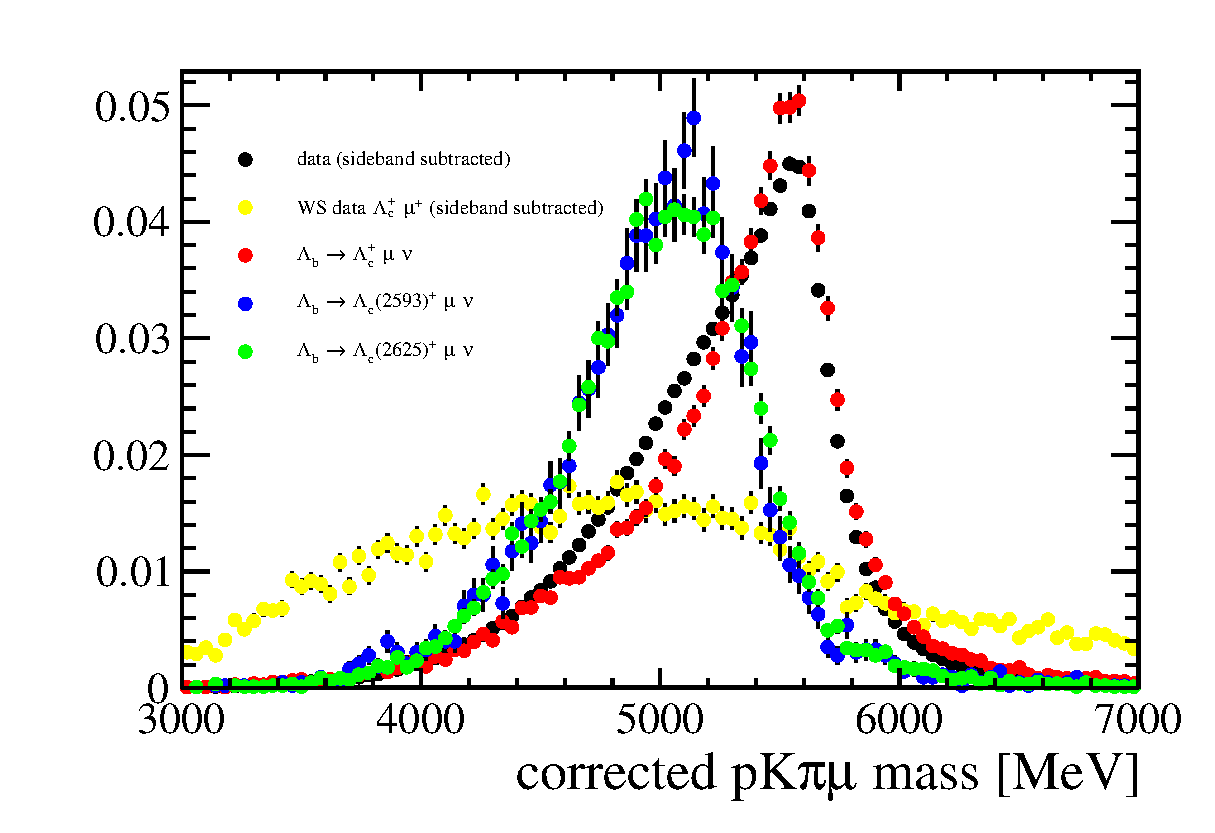
\includegraphics[width=0.49\textwidth]{LbToLc/correctedMass/correctedMass}
	\caption{Comparison of the \pKpi\mun corrected mass for the semileptonic \Lb decays via \Lc, \LcstarRes{(2593)} and \LcstarRes{(2625)} gained from simulation. The black points show the sideband subtracted data distribution. The shape of combinatorial \Lc\mun background (WS events) is shown in yellow.}
	\label{fig:correctedMass_normalisation}
\end{figure}

From figure \ref{fig:correctedMass_normalisation} one can draw the following conclusions:
\begin{itemize}
    \item The corrected \pKpi\mun mass indeed looks different for \Lc and \Lcstar channels.
    \item It is not possible to distinguish between the \LcstarRes{(2595)} and \LcstarRes{(2625)} as their shapes are too similar.
\end{itemize}
The latter conclusion isn't really a problem since the only result of interest is the \LbToLcmunu signal yield. 
A distinction among the excited states isn't needed.
In the fit there will be just a component for both final states.
Having these in mind, the fit procedure is done as follows:
\begin{enumerate}
    \item The data is subtracted by the \pKpi (i.e. \Lc) mass bands.
    \item The corrected \pKpi\mun mass distribution is subtracted by the WS events' distribution.
    \item A fit of the \pKpi\mun mass is performed using the Beeston-Barlow method (see sec. \ref{sec:BeestonBarlow}) to account for uncertainties in the MC corrected mass templates. The fitted components are the \Lc signal yield and one for both excited \Lcstar channels.
    \item For the plotting (see fig. \ref{fig:correctedMass_fit} and a better comparison the WS component is added again.
\end{enumerate}
The results can be seen in figure \ref{fig:correctedMass_fit} and table \ref{tab:fit_correctedMass}. The \LbToLcmunu signal yield \NLc, required for the determination of \R is:
\begin{align*}
    \NLc = (\NLcvalscient \pm \NLcerrscient)\cdot 10^{\NLcexpscient}
\end{align*}
\begin{figure}[hptb]
	\centering
	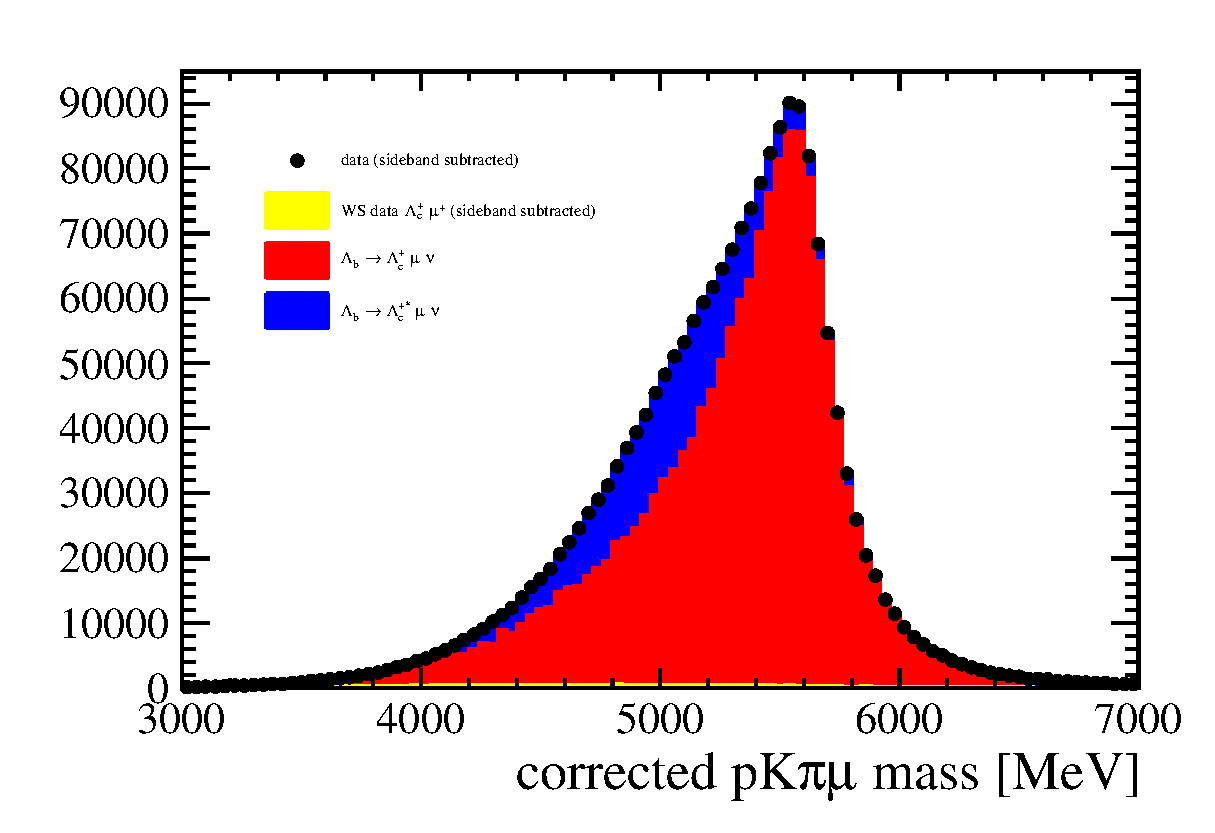
\includegraphics[width=0.49\textwidth]{LbToLc/correctedMass/fit_correctedMass}
	\includegraphics[width=0.49\textwidth]{LbToLc/correctedMass/fit_correctedMass_noBB} \\
	\includegraphics[width=0.49\textwidth]{LbToLc/correctedMass/fit_correctedMass_logscale}
	\includegraphics[width=0.49\textwidth]{LbToLc/correctedMass/fit_correctedMass_noBB_logscale}
	\caption{Fit to the \pKpi\mun corrected mass for the determination of the \LbToLcmunu signal yield. The left plot shows the fitresult with the Beeston-Barlow adjusted templates, the right one the bare templates without any modification. The top row shows the result on a linear, the bottom row on logarithmic scale.}
	\label{fig:correctedMass_fit}
\end{figure}

 
\begin{table}[h]
    \centering
    \caption{Results of the \Lc corrected mass fit.}
    \label{tab:fit_correctedMass}
    $\begin{array}{lr@{\pm}l}
    \hline
    \text{Variable} & \multicolumn{2}{c}{\text{Value}} \\
    \hline
        \text{\Lc candidates \NLc}&(1.5837 & 0.0098) \cdot 10^{6}\\
\text{excited \Lcstar candidates}&(3.849 & 0.087) \cdot 10^{5}\\
\text{combinatoric background}&(3.406 & 0.026) \cdot 10^{4}\\

\hline
\end{array}$
\end{table}
    
